% secciones/implementacion_spark.tex

\section{Implementación en Apache Spark}

Las mismas nueve consultas analíticas se implementaron en PySpark utilizando Spark SQL,
conectado al metastore de Hive mediante \texttt{enableHiveSupport()}. Esto permite operar
sobre las mismas tablas sin duplicar los datos en HDFS.

\subsection{Configuración de la sesión Spark}

Todos los scripts siguen el mismo patrón de inicialización:

\begin{lstlisting}[style=python, caption={Inicialización de SparkSession con soporte Hive}]
from pyspark.sql import SparkSession

spark = SparkSession.builder \
    .appName("nombre_consulta") \
    .enableHiveSupport() \
    .getOrCreate()

spark.sql("USE retail")
\end{lstlisting}

El método \texttt{enableHiveSupport()} conecta Spark al metastore de Hive, permitiendo
acceder directamente a las tablas definidas en la sección anterior sin necesidad de
redefinir esquemas ni recargar datos.

\subsection{Diferencias respecto a HiveQL}

La principal diferencia técnica entre ambas implementaciones es el manejo de
\textit{window functions} en consultas que requieren filtrar por rango dentro de particiones.
HiveQL soporta la cláusula \texttt{QUALIFY} de forma nativa, mientras que Spark SQL no la
implementa. En esos casos se aplica la API de DataFrame de PySpark:

\begin{lstlisting}[style=python, caption={Q5 en Spark: top productos por tienda sin QUALIFY}]
from pyspark.sql import Window
from pyspark.sql.functions import rank

ventas = spark.sql("""
    SELECT s.s_store_name, i.i_product_name,
           SUM(ss.ss_quantity) AS unidades_vendidas,
           SUM(ss.ss_net_paid) AS ingresos_totales
    FROM store_sales ss
    JOIN store s ON ss.ss_store_sk = s.s_store_sk
    JOIN item  i ON ss.ss_item_sk  = i.i_item_sk
    GROUP BY s.s_store_name, i.i_product_name
""")

ventana = Window.partitionBy("s_store_name") \
               .orderBy(ventas["unidades_vendidas"].desc())

resultado = ventas \
    .withColumn("ranking", rank().over(ventana)) \
    .filter("ranking <= 5") \
    .orderBy("s_store_name", "ranking")

resultado.show(truncate=False)
\end{lstlisting}

\begin{figure}[H]
    \centering
    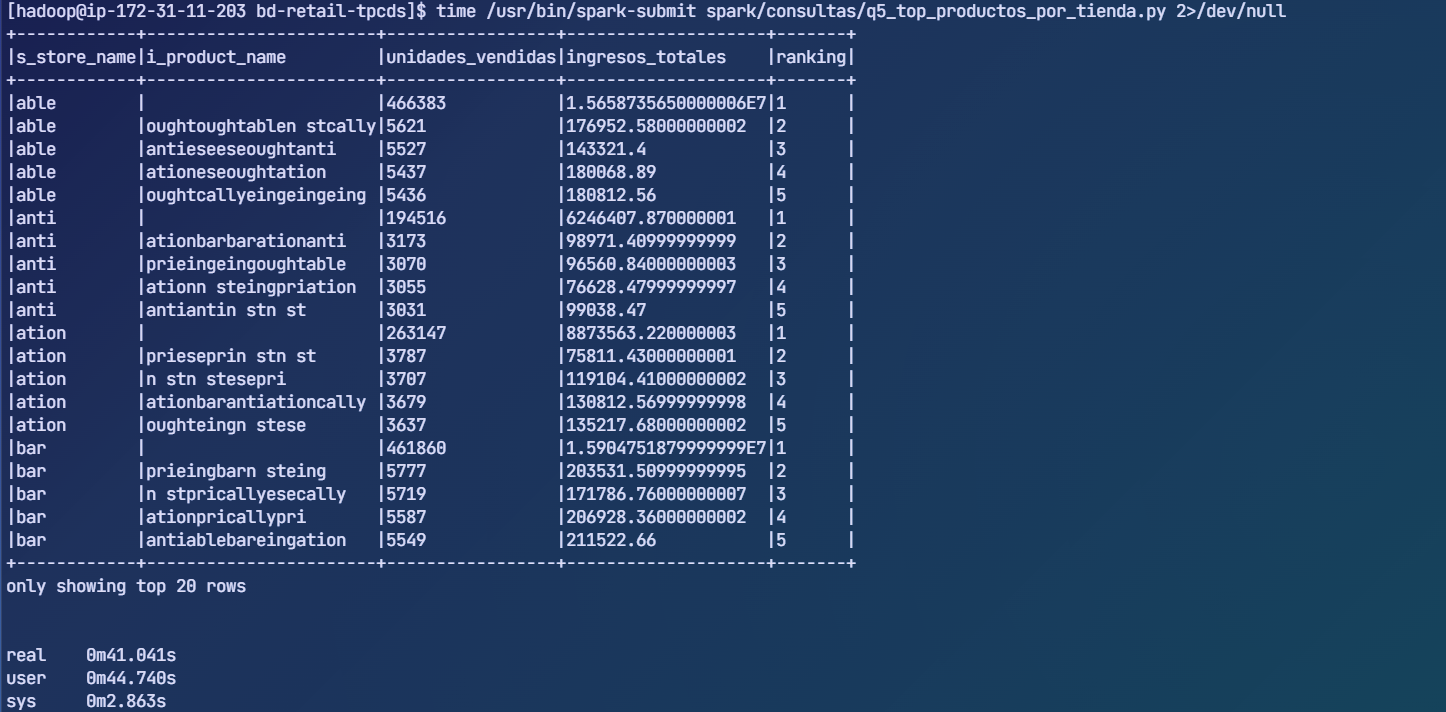
\includegraphics[width=0.85\textwidth]{figuras/spark_q5_resultado.png}
    \caption{Resultado de Q5 en Spark: top productos por tienda.}
\end{figure}

\subsection{Resultados de las consultas en Spark}

\begin{figure}[H]
    \centering
    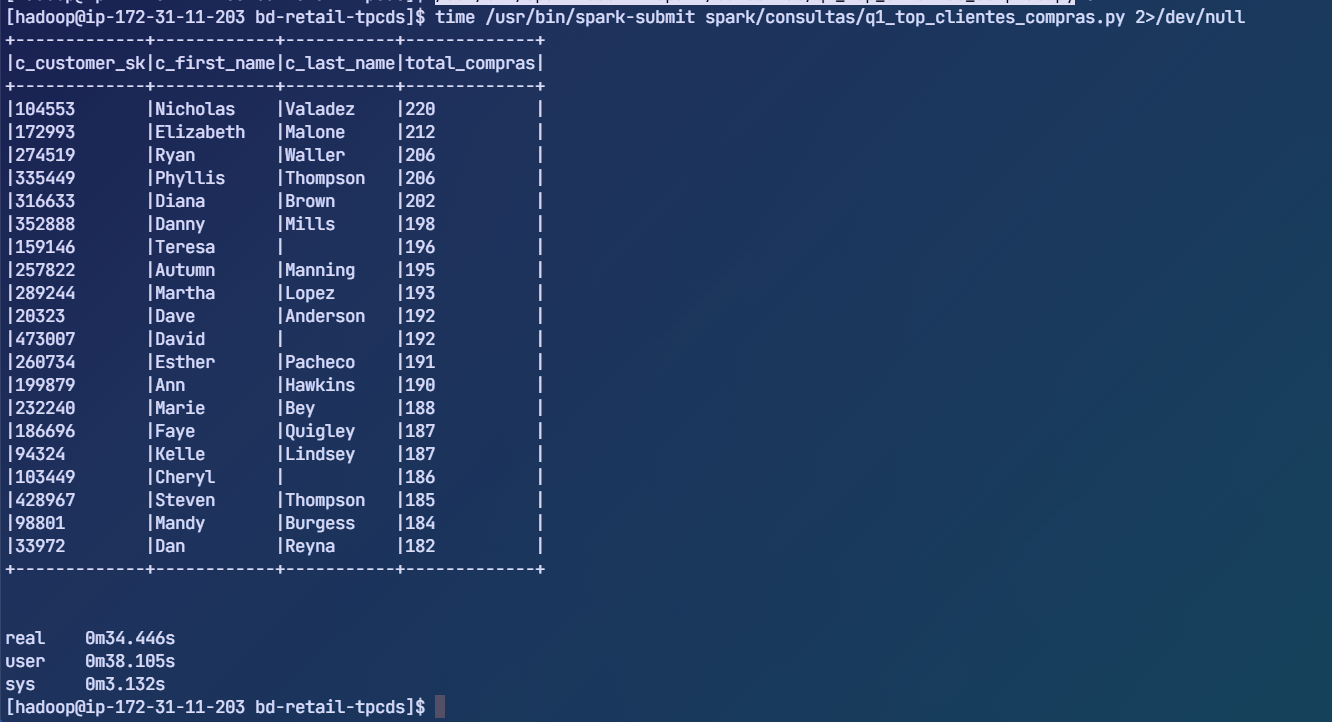
\includegraphics[width=0.85\textwidth]{figuras/spark_q1_resultado.png}
    \caption{Resultado de Q1 en Spark: top 20 clientes por número de compras.}
\end{figure}

\begin{figure}[H]
    \centering
    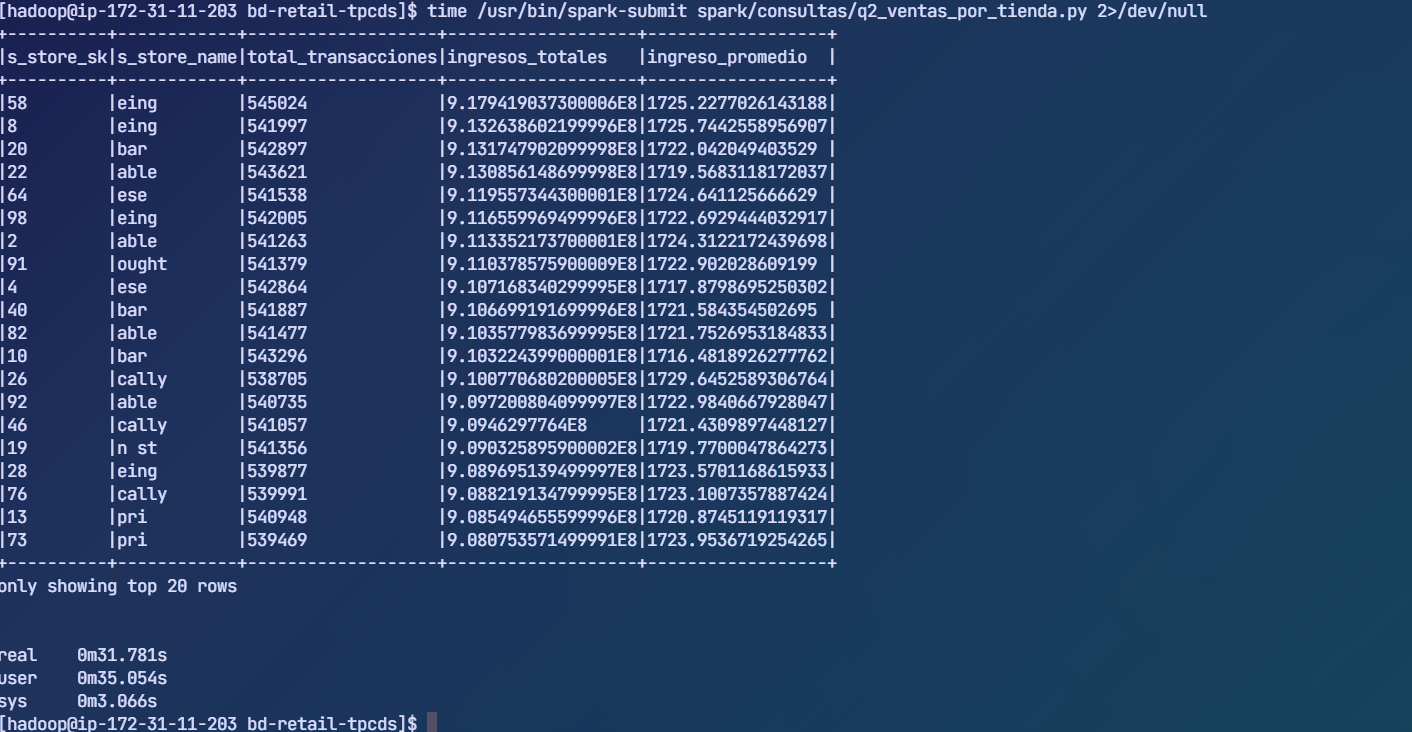
\includegraphics[width=0.85\textwidth]{figuras/spark_q2_resultado.png}
    \caption{Resultado de Q2 en Spark: ventas por tienda.}
\end{figure}

\begin{figure}[H]
    \centering
    \includegraphics[width=0.85\textwidth]{figuras/spark_q3_resultado.png}
    \caption{Resultado de Q3 en Spark: ventas por mes.}
\end{figure}

\begin{figure}[H]
    \centering
    \includegraphics[width=0.85\textwidth]{figuras/spark_q9_resultado.png}
    \caption{Resultado de Q9 en Spark: ranking mensual de tiendas.}
\end{figure}
